%% thesisclass.sty
%% Copyright 2022 D.Piciocchi
%
% This work may be distributed and/or modified under the
% conditions of the LaTeX Project Public License, either version 1.3
% of this license or (at your option) any later version.
% The latest version of this license is in
%   http://www.latex-project.org/lppl.txt
% and version 1.3 or later is part of all distributions of LaTeX
% version 2005/12/01 or later.
%
% This work has the LPPL maintenance status 'maintained'.
% 
% The Current Maintainer of this work is D. Piciocchi.
%
% This work consists of the files masterthesis.cls, thesisclass.sty,
% Master_Thesis.tex, Bibliography.bib, glossary.tex, compilepdf.sh,
% the Chapters folder containing titlepage.tex, titlepage.pdf,
% abstract.tex, acknowledgements.tex, instructions.tex
% 

%%%%%%%%%%%%%%%%%%%%%%%%%%%%%%%%%%%%%%%
%%%%%%%%%%%%%% MAIN FILE %%%%%%%%%%%%%%
%%%%%%%%%%%%%%%%%%%%%%%%%%%%%%%%%%%%%%%

%%%%% MAIN FILE %%%%%%%%%%

\documentclass[12pt,a4paper,twoside,onecolumn,openright]{thesisclass}

%%%%%% METADATA CREATION %%%%%%%%%%%%%%

% This is done in this way since the pdfx package is being used. 
% If in any case you need to drop that, you will also add hyperref and metadata creation can be done with that as well. Otherwise, edit the xmpdata file directly.

\begin{filecontents*}[overwrite]{\jobname.xmpdata}
    \Title{A class to typeset your Master Thesis}
    \Author{Diego Piciocchi}
    \Language{british}
    \Subject{This document contains all the information on how to use this LaTeX class.}
    \Keywords{latex\sep class\sep thesis}
\end{filecontents*}

%%%%% BIBLIOGRAPHY SOURCE FILE %%%%%%%%%

\addbibresource{Bibliography.bib}

%%%%% MAKING GLOSSARY %%%%%%%%%

\makeglossaries
\loadglsentries{glossary}

%%% GRAPHICS PATH AND DOC SPECIFIC COMMANDS %%%%

\graphicspath{{images}%
{images/frontmatter}%
}

%%%%%%%%%%%%%%%%%%%%%%%%%%%%%%%%%%%%%%%%
%%%%%%%% DOCUMENT BEGINNING %%%%%%%%%%%%
%%%%%%%%%%%%%%%%%%%%%%%%%%%%%%%%%%%%%%%%


\begin{document}

% FRONT MATTER 

\frontmatter %Denotes Frontmatter beginning

\pagenumbering{roman} % Roman page numbering prior to the start of the thesis

% For now, the title page and dedication are included as a separate pdf to allow setting different margins for it in an easy way.

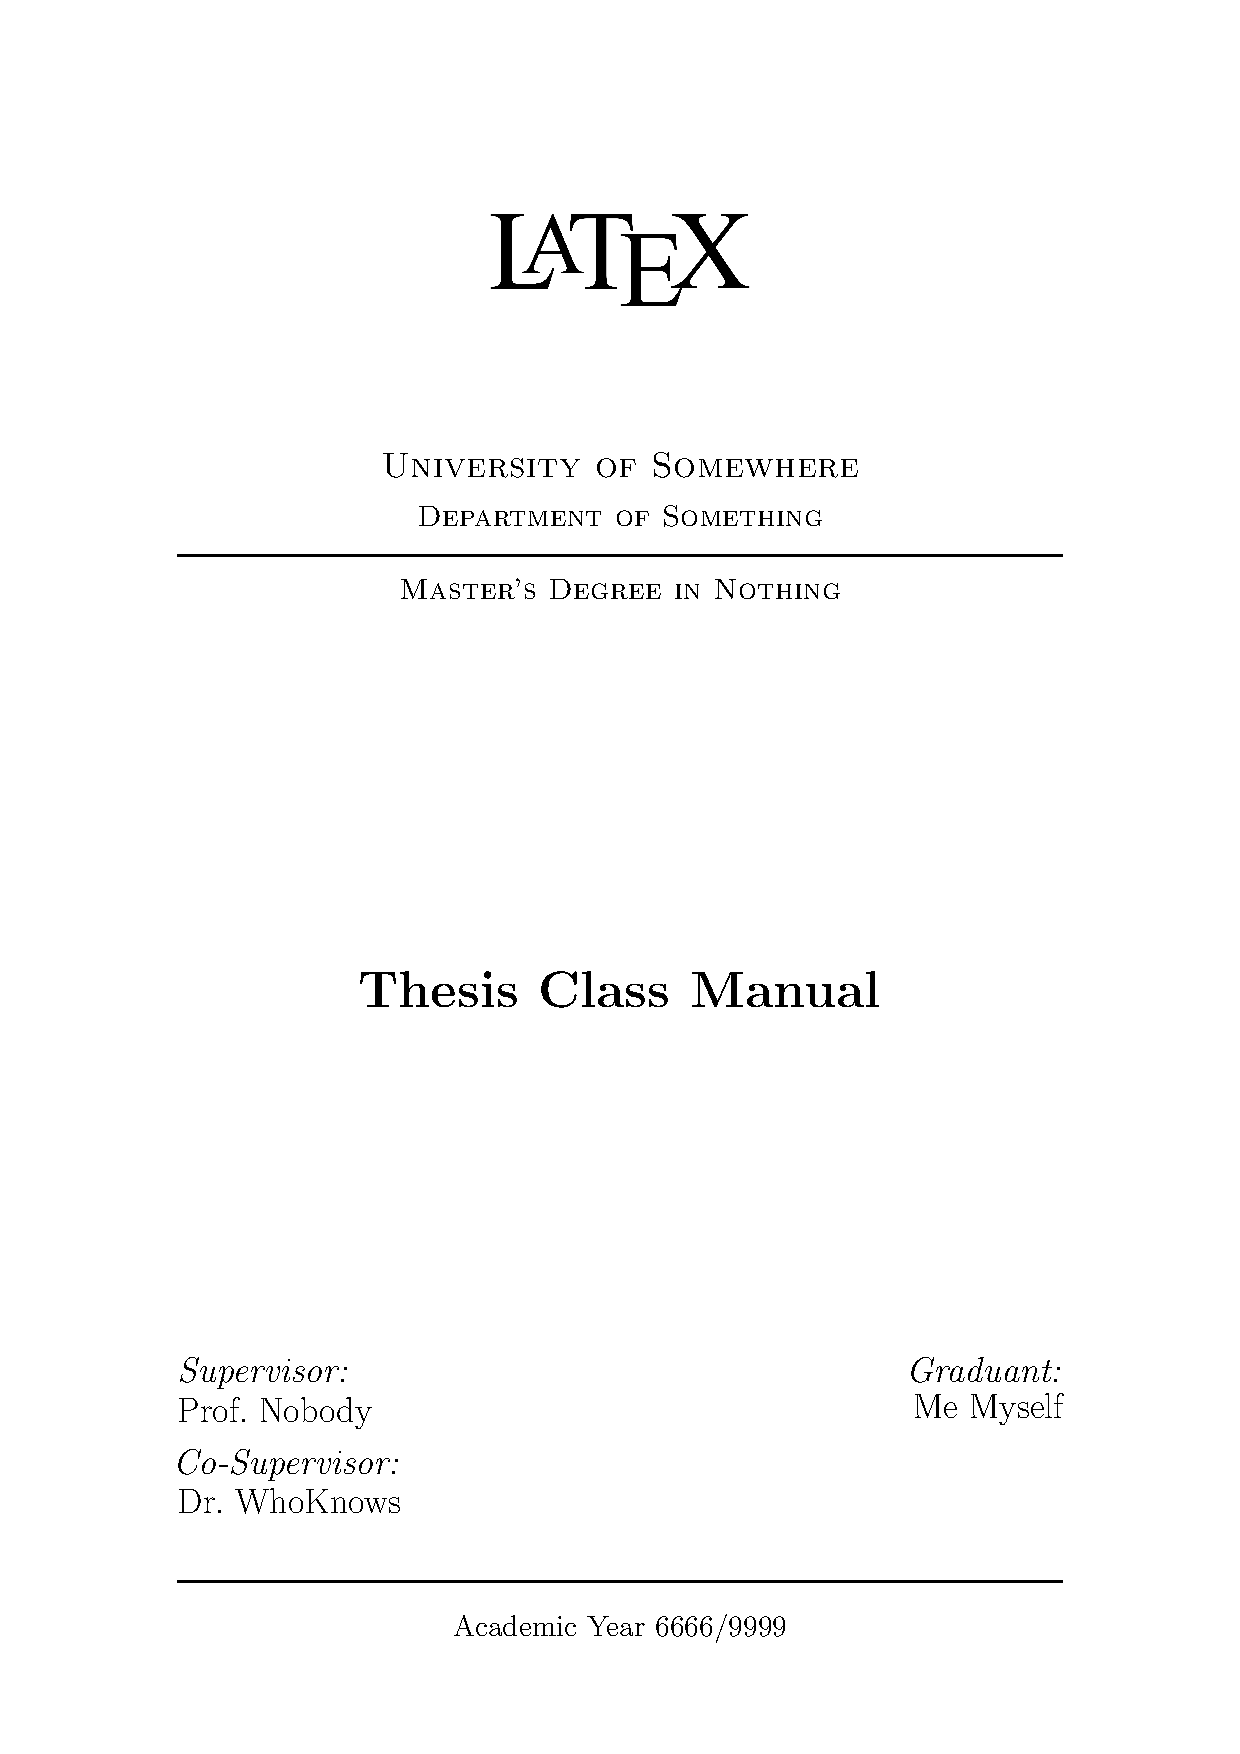
\includepdf[pages=1-3]{Chapters/Frontmatter/titlepage.pdf}
\cleardoublepage
\pagestyle{plain} % Suppress headers for the pre-content pages
%% acknowledgements.tex
%% Copyright 2022 D.Piciocchi
%
% This work may be distributed and/or modified under the
% conditions of the LaTeX Project Public License, either version 1.3
% of this license or (at your option) any later version.
% The latest version of this license is in
%   http://www.latex-project.org/lppl.txt
% and version 1.3 or later is part of all distributions of LaTeX
% version 2005/12/01 or later.
%
% This work has the LPPL maintenance status 'maintained'.
% 
% The Current Maintainer of this work is D. Piciocchi.
%
% This work consists of the files masterthesis.cls, thesisclass.sty,
% Master_Thesis.tex, Bibliography.bib, glossary.tex, compilepdf.sh,
% the Chapters folder containing titlepage.tex, titlepage.pdf,
% abstract.tex, acknowledgements.tex, instructions.tex
% 

%%%%%%%%%%%%%%%%%%%%%%%%%%%%%%%%%%%%%%%
%%%%%%%%%%% ACKNOWLEDGEMENTS %%%%%%%%%%
%%%%%%%%%%%%%%%%%%%%%%%%%%%%%%%%%%%%%%%

\pdfbookmark[1]{Acknowledgements}{Acknowledgements} % Bookmark name visible in a PDF viewer

\chapter*{Acknowledgements}

Thank you guys!!

\vfill

%% abstract.tex
%% Copyright 2022 D.Piciocchi
%
% This work may be distributed and/or modified under the
% conditions of the LaTeX Project Public License, either version 1.3
% of this license or (at your option) any later version.
% The latest version of this license is in
%   http://www.latex-project.org/lppl.txt
% and version 1.3 or later is part of all distributions of LaTeX
% version 2005/12/01 or later.
%
% This work has the LPPL maintenance status 'maintained'.
% 
% The Current Maintainer of this work is D. Piciocchi.
%
% This work consists of the files masterthesis.cls, thesisclass.sty,
% Master_Thesis.tex, Bibliography.bib, glossary.tex, compilepdf.sh,
% the Chapters folder containing titlepage.tex, titlepage.pdf,
% abstract.tex, acknowledgements.tex, instructions.tex
% 

%%%%%%%%%%%%%%%%%%%%%%%%%%%%%%%%%%%%%%%
%%%%%%%%%%%% ABSTRACT FILE %%%%%%%%%%%%
%%%%%%%%%%%%%%%%%%%%%%%%%%%%%%%%%%%%%%%


\pdfbookmark[1]{Abstract}{Abstract} % Bookmark name visible in a PDF viewer

\chapter*{Abstract}
These are the instructions on how to properly use the template. I recommend you rename this pdf file before recompiling so you can keep it somewhere and have the instructions in case you need them.
\begin{center}
	\today
\end{center}

\vfill

\cleardoublepage

% Table of Contents, List of Tables and List of Figures

\tableofcontents*
%\listoftables*
%\listoffigures*

%% MAIN MATTER 

\mainmatter
\pagestyle{ruled}

zz%% thesisclass.sty
%% Copyright 2022 D.Piciocchi
%
% This work may be distributed and/or modified under the
% conditions of the LaTeX Project Public License, either version 1.3
% of this license or (at your option) any later version.
% The latest version of this license is in
%   http://www.latex-project.org/lppl.txt
% and version 1.3 or later is part of all distributions of LaTeX
% version 2005/12/01 or later.
%
% This work has the LPPL maintenance status 'maintained'.
% 
% The Current Maintainer of this work is D. Piciocchi.
%
% This work consists of the files masterthesis.cls, thesisclass.sty,
% Master_Thesis.tex, Bibliography.bib, glossary.tex, compilepdf.sh,
% the Chapters folder containing titlepage.tex, titlepage.pdf,
% abstract.tex, acknowledgements.tex, instructions.tex

\chapter[Instructions][Instructions]{Instructions}
\label{Instructions}

In the following, the instructions and features concerning this \texttt{thesisclass} \LaTeX\hspace{2pt} class are discussed. As this class is based on the \texttt{memoir} class, it is recommended to read the manual \cite{memoirman} \footnote{\url{http://tug.ctan.org/tex-archive/macros/latex/contrib/memoir/memman.pdf}} in order to be able to modify the default settings.

\section{Main Features}

The main goal of the class is to provide a customisation of \texttt{memoir} which is ready to use for typesetting a thesis in Physics or Mathematics in English. This means that the following features are prioritized

\begin{itemize}
\item Automated compilation of the full document
\item A decent default set of packages
\item An appropriate typographic style
\item A tidy, commented and therefore user-friendly code/template layout 
\item Best amount of options, inherited from memoir
\end{itemize}

\section{How to Compile}

This document was designed, tested and compiled in Linux (using bash as a shell). Therefore, if you work in the same environment, you can take advantage of the \texttt{bash} script included in the project files. The first time, you have to run

\begin{lstlisting}[language=bash,caption={bash version}]

chmod +x compilepdf.sh
./compilepdf.sh thesisclass

\end{lstlisting}

And after the first time only the second line is needed. The content of the script is basically the following

\begin{lstlisting}[language=bash,caption={bash version}]
#!/bin/bash  

cd Chapters/Frontmatter
pdflatex titlepage
cd ..
cd ..

pdflatex $1 
makeglossaries $1 
biber $1
pdflatex $1 

\end{lstlisting}

The first (and only) positional variable is the title of the main \TeX\hspace{2pt} file you are using.The script simply goes to the directory containing the titlepage file and compiles it. Then, it goes back to compile the main document. These are the same steps you will need to run if you compile the document manually. Here is an example:

\begin{lstlisting}[language=bash,caption={bash version}]

cd Chapters/Frontmatter
pdflatex titlepage
cd ..
cd ..

pdflatex thesisclass
makeglossaries thesisclass 
biber thesisclass
pdflatex thesisclass 

\end{lstlisting}
  

With a full TexLive installation, you won't experience problems due to missing packages. With subsets of TexLive, your mileage may vary. You can troubleshoot issues related to this looking for packages on CTAN or moving to a full installation. In a similar way, you should be able to compile the documant on MacOS or Windos terminals (they should allow to run bash scripts as well). Compatibility with environments (IDE like) which compile the document automatically could work, but this will probably depend on user configuration. Tests are planned in this regard. The template also works in Overleaf. However, compile time is long and if the progect becomes larger you may exceed the available compile time. 

\section{Included Packages}

The template should include everything you need to read and prpduce coherent and nice looking text in english. Dummy text, quotations and including pdf pages are supported. All the AMS packages are included, which should be enough to typeset math correctly. I also addes \texttt{mathrsfs} for \textit{scr} fonts in math (like $\mathscr{H}$) and \texttt{mathtools} to extend the functionality of \texttt{amsmath}. \texttt{empheq} allows the user to highlight equations. I also added the \texttt{physics} and \texttt{siunitx} packages for physical objects (like $\bra{\psi}$, $\ket{\psi}$ and $\mel{\psi}{\mathscr{H}}{\phi}$ and others) and SI units. Packages to include and customise tables are available. The default ones are the recommended "must have" for publication/book quality tables, but there are many more. Packages to include external graphics (plots of data etc.) are available. \texttt{tikz} is available with a decent set of libraries and \texttt{pgfplots} in case you want to create schematics or plot functions directly in the document. In case you need to add extra packages, you can either use the \texttt{\\RequirePackage} command in \texttt{thesisclass.sty} (for "permanent" use in the class) or using \texttt{\\usepackage} in the document preamble. The same holds for the definitions of your own commands or environments. 

\section{Typographic Aspects}

Some personal choices were made with respect to the typographic layout, and the result is what you see in this manual. All the configuration for the size and position of the text block on the page has been performed according to the instructions contained in \cite{memoirman} and are found in \texttt{thesisclass.sty}. Here, I briefly outline my choices and the reasons behind them. First of all, a well engineered page design should not be noticeable (and I hope this one is not...). It should not scream "look how well I organised it!" at every page. It should simply make the document easy and comfortable to read and thus it should almost be unnoticed. One way to achieve this is the choice of an appropriate line width. As far as i could find out, for single column documents the ideal number of characters per line is in a range going between 50 and 75, with the ideal value being 66. Of course where you choose to place the actual mean value in the documents you make depends on the choice of typeface and font. In this manual, I used 12pt Palatino and edited the width of the block to obtane a mean value for the line length of 60 characters. I think this is a good choice in terms of readability. I chose Palatino over the maybe more widespread Times New Roman as I have no constraint on the length of my document, and i thus do not intend to pack the text tooo tightly. I have left a commented option to switch to Times (or Utopia) in \texttt{thesisclass.sty}. Maybe if you choose to use this option you will need to adjust the block size. As far as positioning on the page goes, I personally like an asymmetric layout (amongst other advantages, it leaves room for the reader to take notes on printed versions). Be careful that if you choose to do so, the asymmetry between left and right margins \textbf{needs} to be evident, in order to avoid a sense of "there's something wrong here" in the reader. In this case, the outer margin is 1.6 ytimes the inner margin. The height of the block is fixed at 634pts. I also chose to use the \texttt{microtype} package for better thext appearance. The default values of my choice can be found in \texttt{thesisclass.sty} and tinkered with at will. The reader is warned: do this with care as you interfere with the decisions of the typeface designers (who chose the parameters carefully). Now, a common choice when using 1.5 column layouts similar to mine is to leave a margin that is wide enough to include content, like notes, figures and tables. This is for example the strategy E.Tufte uses in his books and several \LaTeX\hspace{2pt} classes have been designed based on this. There is a strong argument behindthis choice: it allows to not break the flow text by placing things that "help" the content expressed by words on the sides of the page. The results are often exceptionally good. One indeed can modify this class and define environments to obtain similar results (but at that point it might be more efficient to use one of the many available classes). I really like the "narrower" column of Tufte's design, with lines that are easy to read. I used it many times and I partly reproduced it here. However, this template is explicitly designed for a Thesis in Physics. In this type of document figures and tables are not just "helpful" content. They more likely become the protagonist of the page when they appear and are the main content to look at. Hence, they basically always deserve more space. Then, the wider margins of Tufte's layout would not actually be efficiently used for their designed purpose. Hence, my choice of modifying that design. Notice that Tufte's layout can often efficiently display even full page figures, and for many users that choice may be better (I advise the reader to try that out as well and make a choice).

\subsection{Pagestyle, Titles}

For the pagestyle, i chose the \texttt{ruled} option from memoir, which provides a heading with a line containing the chapter name on even pages and the section name on odd ones. One could switch to an even simppler layout like \texttt{plain} editing \texttt{thesisclass.sty}. For the titles of chapters, i chose the predefined \texttt{madsen} style from meoir. I left several good options in \texttt{thesisclass.sty}, and one could even make custom titles if needed.

\section{Bibliography, Glossary, Contents and Hyperlinks}

The document is made to also print out the table of contents, list of figures and list of tables at the beginning of the document. In this manual, you do not see lists of figures and tables since they are empty and have been commented out in \texttt{thesisclass.tex}.The options for these are left very close to the defaults for the memoir class and can be found in \texttt{thesisclass.sty}. The bibliography is prepared using \texttt{biblatex} with \texttt{biber} as a backend. The options used to print the bibliography and display the citations can be easily found and modified in \texttt{thesisclass.sty}. Hyperlinks are enabled via the \texttt{hyperref} package (see later) and some easy options have been chosen for the color of links. Chapters, sections and subsections are also bookmarked. 

\section{PDF Standard}

The \texttt{pdfx} package has been used to produce a file that is compliant to the PDF/A standard. As an option, you can choose between levels of compliance from 1 to 4. Sadly, only b level files can be produced. The University of Trento requires 1 and this i set the compliance to be PDF/A-1b (the closest to the one required). Notice that this package also loads \texttt{hyperref} and \texttt{xcolor}, so there is no need to call them separately and theis options can be set as usual. Please be aware that the \texttt{pdfx} package may cause problems with bookmarks when using mathematical symbols in titles of sections and similar. In this case, you could call \texttt{hyperref} and \texttt{xcolor} separately and avoid this package, at the cost of losing the compliance. Metadata associated to the file are produced in the preamble of \texttt{thesisclass.tex}

\section{Final Notice}

Notice that this class and the corresponding manual are both under development and that I do not have a lot of time. Mistakes are to be expected and I would appreciate it if you were to report them to me. You can write an email at \texttt{diegopiciocchi@studenti.unitn.it} 








\cleardoublepage

%% BACK MATTER 

\backmatter

% Appendices. Uncomment to insert them
% \part*{Appendices}

% \chapter[Appendix A][Appendix A]{Appendix A }
\label{AppendixA}

Here, one can write an appendix!


% Glossary, list of terms

\glsaddall % this adds all entries to the glossary
\printglossary[type=\acronymtype, toctitle=Acronyms]
\printglossary[title=List of Terms, toctitle=Glossary]

% Bibliography

\cleardoublepage

\printbibliography[title={Bibliography}]

\end{document}

